This Chapter has introduced the idea of creating Procedures within your program's code. These procedures can be used to implement the different tasks that you want your program to perform. 

This Section will help you answer the following questions:
\begin{itemize}
  \item How can I visualise the Procedures within a Program?
  \item What happens when my Procedures are called?
\end{itemize}

\subsection{Visualising Procedures in Morse Calling} % (fold)
\label{sub:visualising_morse_calling}

When you are writing the code, the internal details of how a Procedure works are important. But, it is equally important to be able to picture how these procedures interact within the Program as a whole. One technique for visualising this is to draw a \textbf{Structure Chart}.

A \emph{Structure Chart} is a diagram that has two elements: rectangles representing the procedures in your code, and arrows representing calls. The Structure Chart for the Morse Calling program is shown in Figure \ref{fig:procedure-decl-morsecalling-structure}. In this you can see that the Morse Calling program has four main procedures that implement its functionality, in addition to the Program's main logic: the \texttt{Signal C}, \texttt{Signal Q}, \texttt{Long Signal}, and \texttt{Short Signal} procedures. It also shows that the program's main logic calls \texttt{Signal C} and \texttt{Signal Q}, that \texttt{Signal C} calls \texttt{Long Signal} and \texttt{Short Signal}, as does \texttt{Signal Q}.

\begin{figure}[htbp]
   \centering
   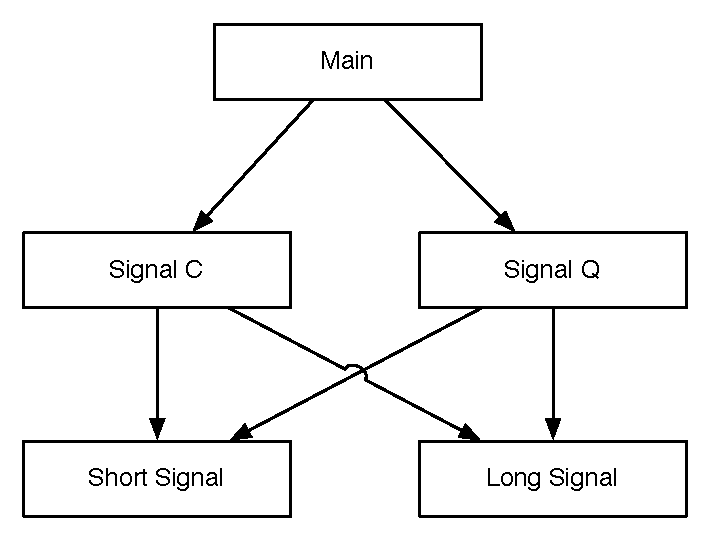
\includegraphics[width=0.75\textwidth]{./topics/procedure-decl/diagrams/MorseCallingStructureChart} 
   \caption{Structure Chart showing the Procedures in Morse Calling}
   \label{fig:procedure-decl-morsecalling-structure}
\end{figure}

The rectangles in the Structure Chart represent the Procedures. As the name of the procedure should reflect its task/actions this means that the reader of the diagram can get some insight into what the program is doing, and how it is achieving its tasks. From Morse Calling's Structure Chart you can see that the program is Signalling the character's \emph{C} and \emph{Q}, which internally use \emph{Long} and \emph{Short} signals to achieve their tasks.

The arrows in the Structure Chart show Procedure Calls. The arrow from the \texttt{Signal C} procedure to \texttt{Long Signal} tells us that somewhere in the code for \texttt{Signal C} there is one or more calls to \texttt{Long Signal}. There is no indication of the order, or frequency, of these calls. Its just simply saying that \texttt{Signal C} calls \texttt{Long Signal}.

The Structure Chart is useful for getting an overall picture of how the program is structured. It can help the designer communicate such things as \emph{What Procedures are there in this Program?} and \emph{How are these Procedures related to each other?} It helps developers new to the project to get a feeling for how the code is distributed within the solution, and to know where the core logic can be found. It also provides a means of determining the impact of changing the functionality of the tasks in the Program. For example, if you change how \texttt{Long Signal} works that may impact on \texttt{Signal C} and on \texttt{Signal Q}. Any changes you made here would mean you needed to test that \texttt{Signal C} and \texttt{Signal Q} still worked as expected.

\bigskip

The Structure Chart is a great communication tool for getting an overall picture of how a solution fits together, but it only shows the \textbf{static structure}. Communicating things about the code, but not things about how the code executed. An effective designer will want to communicate both the \emph{static structure}, as well as the \textbf{dynamic behaviour} of the solution. To communicate these details you need to look for complementary techniques.

% sub:visualising_morse_calling (end)

\subsection{Visualising Procedure Calls in Morse Calling} % (fold)
\label{sub:visualising_procedure_calls_in_morse_calling}

The Structure Chart communicates the static structure of the solution, showing the Procedures and their relationships but lacking any details on how this structure works dynamically. This dynamic information can be captured in a \textbf{Sequence Diagram}, which works together with the Structure Chart to complete the overview of the program's structure and dynamic behaviour.

Figure \ref{fig:procedure-decl-morsecalling-sequence} shows the \emph{Sequence Diagram} for the Morse Calling program. This shows the \emph{Procedure Calls} that will occur within an execution of the Program's code. The Sequence Diagram shows the order in which Procedure Calls occur, with time travelling down the page and the calls travelling across. 

\begin{figure}[htbp]
   \centering
   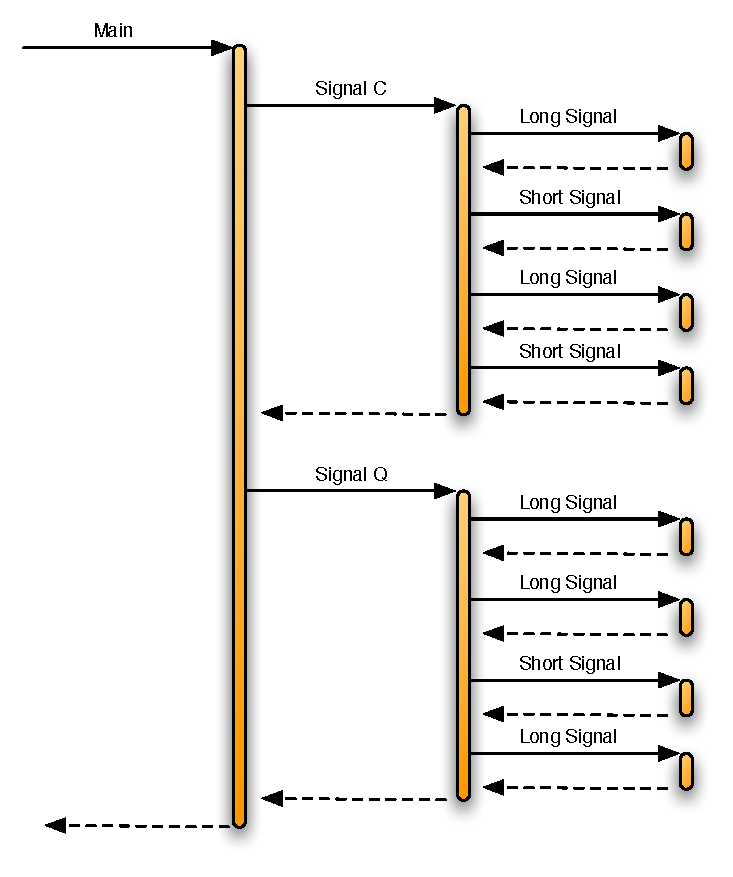
\includegraphics[width=0.75\textwidth]{./topics/procedure-decl/diagrams/MorseCallingSequenceDiagram} 
   \caption{Sequence Diagram for Morse Calling}
   \label{fig:procedure-decl-morsecalling-sequence}
\end{figure}

You start reading this diagram from the top, with each arrow representing the call to a Procedure, and the thin vertical rectangles representing the time taken for the called procedure to complete its task. Reading the Sequence Diagram for Morse Calling you can see that the first thing to occur is the \texttt{Main} body of the program's code is started. The arrow from the far left indicates that something, in this case being the user launching the program, starts this code running.

The first thin vertical rectangle is the Program's main instructions, and its first action is to call \texttt{Signal C} as shown by the arrow pointing to the second vertical bar. This is our first Procedure Call, the program's instructions call \texttt{Signal C}. Notice that at this point there are two vertical bars. These represent the two frames on the Stack, and show us that when \texttt{Signal C} finishes the execution will return to the Program's main instructions.

Within \texttt{Signal C} the first action is to call \texttt{Long Signal}, as shown be the arrow. Time-wise this is the second procedure call. First the Main code called \texttt{Signal C}, which in turn called \texttt{Long Signal}. The details on the diagram show us that \texttt{Long Signal} does not call any other procedures that we created. Notice that we have avoided putting in the call to the output procedure to allow us to focus on the Procedures we have created. At this point there are three frame's on the Stack, the first for the \texttt{Main} code, second for \texttt{Signal C}, and third for \texttt{Long Signal}. You can see these if you turn your head on the side. Notice the notice that the vertical bars will mirror the stack.

As \texttt{Long Signal} does not call any other Procedures that we created there are no calls coming out from this procedure's execution. The actions within this code will be performed, and then \texttt{Long Signal} will end. This is shown by the ending of the vertical bar, and a dashed returning arrow showing where the code returns to. This tells us that when \texttt{Long Signal} ends at this point, the computer returns to execute the next instruction in \texttt{Signal C}.

The next instruction in \texttt{Signal C} is the call to \texttt{Short Signal}. Once again this is shown with the calling arrow, and a vertical bar is added to show the steps of the \texttt{Short Signal} executing. \texttt{Short Signal} does not call any other Procedures we created so it ends without any additional calls occurring, and control returns to \texttt{Signal C}.

This process continues, with the diagram showing that \texttt{Long Signal} is called again followed by a call to \texttt{Short Signal}, and then \texttt{Signal C} ends. At this point control returns to the Program's main code, where the next call starts \texttt{Signal Q} running. Within \texttt{Signal Q} you can see two calls to \texttt{Long Signal}, followed by a call to \texttt{Short Signal}, and a final call to \texttt{Long Signal}. When the final call to \texttt{Long Signal} ends this marks the end of the \texttt{Signal Q} procedures, and the end of the Program's instructions as a whole.

As you can see from the above text the Sequence Diagram communicates a large amount of detail in a relatively small space. Trying to communicate the calling sequence in words is far harder than doing so in a diagram like this. The Sequence Digram allows software designers to communicate the dynamic behaviour of a software solution.

One issue with a Sequence Diagram is that it can quickly become very large if you use it to try and explain all of the actions within a program. As the complexity of your programs grow you will see that it becomes more and more difficult to try to communicate all of the program's behaviour in a single diagram. Instead of trying to communicate the entire program's behaviour, effective Software Designers will use Sequence Diagrams to communicate important details that may be missed otherwise. Focusing on areas where the interaction between the procedures is particularly important. As you progress as a Software Developer see if you can use these diagrams to effectively communicate important points in your designs.

\bigskip

Together \emph{Structure Charts} and \emph{Sequence Diagrams} allow Software Designers to communicate the static structure and dynamic behaviour of their designs. As a software developer you will need to understand how to read these diagrams, and use them to communicate your designs decisions.

% subsection visualising_procedure_calls_in_morse_calling (end)

\subsection{Procedure Calls in Action} % (fold)
\label{sub:procedure_calls_in_action}

The Sequence Diagram gives you a way of visualising what happens at run time, but let us return to our virtual computer and see how these actions actually work within the computer. 

\begin{enumerate}
  \item \nameref{ssub:morse_calling_is_loaded_into_memory}
  \item \nameref{ssub:signal_c_is_called}
  \item \nameref{ssub:long_signal_is_called}
  \item \nameref{ssub:control_returns_to_signal_c}
  \item \nameref{ssub:short_signal_is_called}
  \item \nameref{ssub:short_signal_ends}
\end{enumerate}

\clearpage
\subsubsection{Morse Calling is Loaded into Memory} % (fold)
\label{ssub:morse_calling_is_loaded_into_memory}

When the program is launched the Operating System loads the code for Morse Calling into memory, and starts it executing in the Program's entry point. 

\begin{figure}[htbp]
   \centering
   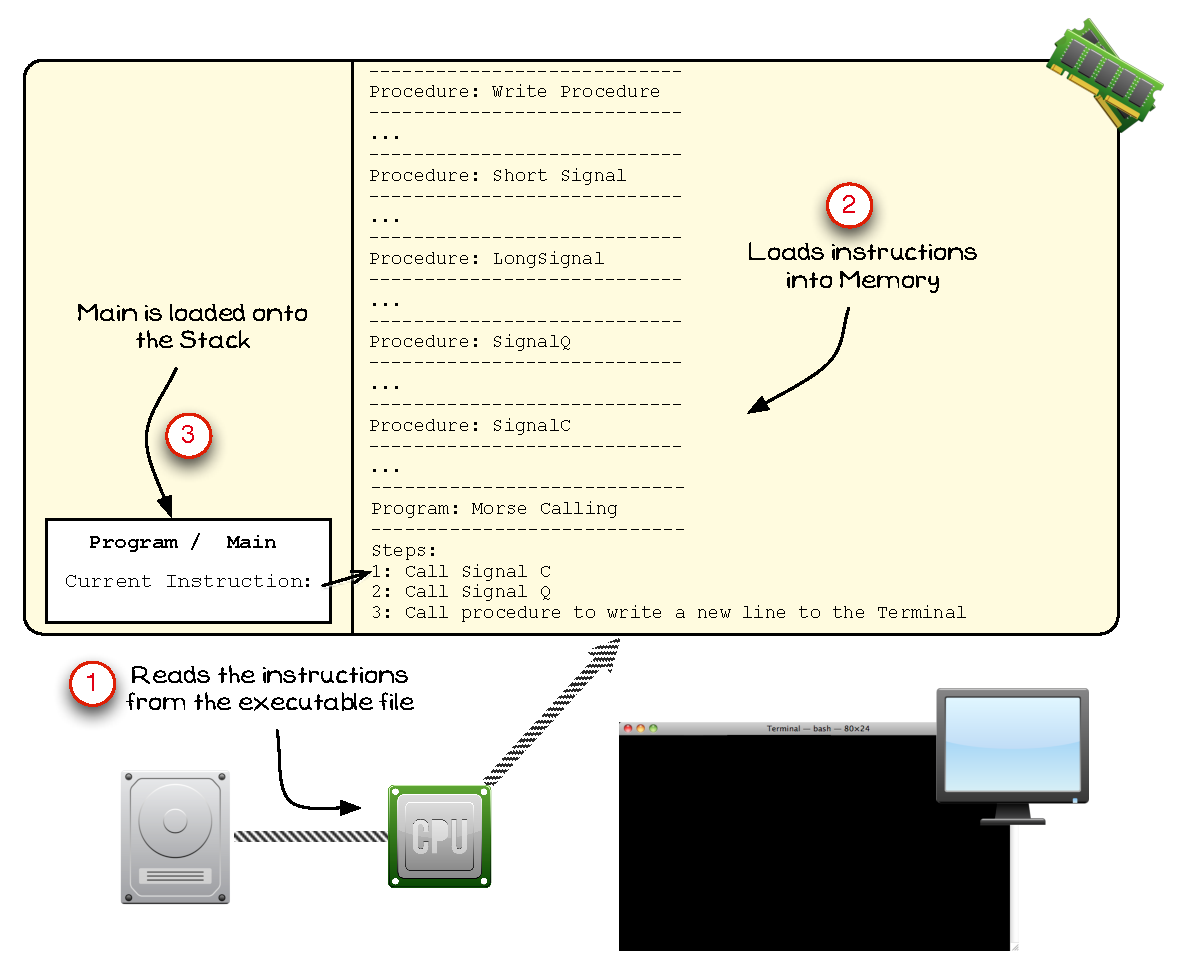
\includegraphics[width=\textwidth]{./topics/procedure-decl/images/ProcExe1} 
   \caption{The Operating System loads the code for Morse Calling into memory}
   \label{fig:procedure-decl-visualise-morsecalling-1}
\end{figure}

\mynote{
\begin{itemize}
  \item In Figure \ref{fig:procedure-decl-visualise-morsecalling-1} the indicated areas show the following:
  \begin{enumerate}
    \item The Operating System reads the code from the Morse Calling executable.
    \item This code is then loaded into the Program's memory.
    \item A frame is added to the Stack for the entry point, the start of the program's instructions.
  \end{enumerate}
  \bigskip
  
  \item The memory for the program is divided into areas for the \textbf{stack}, and the \textbf{code}.
  \item Only part of the Program's code is shown in Figure \ref{fig:procedure-decl-visualise-morsecalling-1}, but in reality all of the program's code is loaded into memory.
\end{itemize}
}

% subsubsection morse_calling_is_loaded_into_memory (end)

\clearpage
\subsubsection{Signal C is Called} % (fold)
\label{ssub:signal_c_is_called}

The first action in the Program's code is a procedure call that starts the code in \texttt{Signal C} running. 

\begin{figure}[htbp]
   \centering
   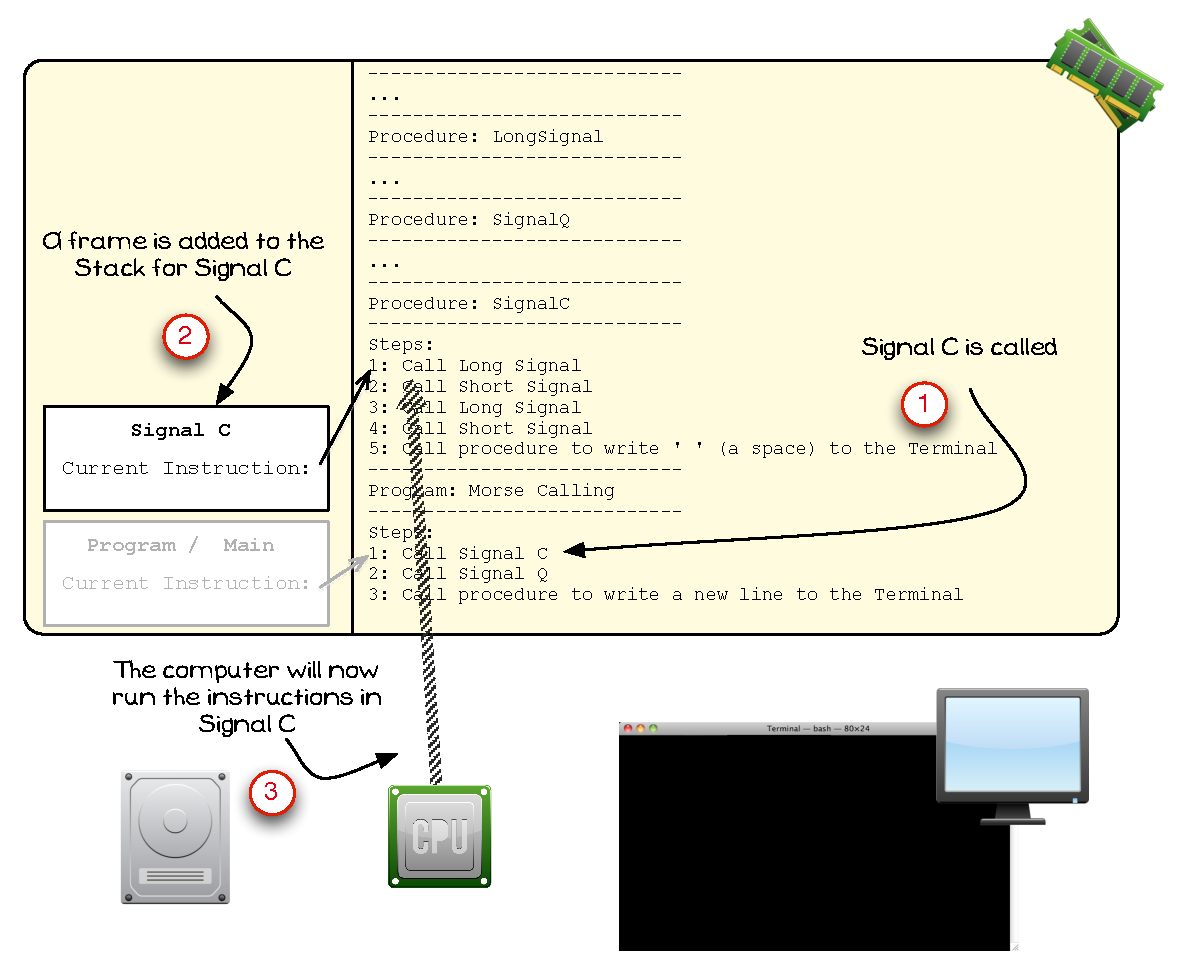
\includegraphics[width=\textwidth]{./topics/procedure-decl/images/ProcExe2} 
   \caption{The first instruction calls \texttt{Signal C}}
   \label{fig:procedure-decl-visualise-morsecalling-2}
\end{figure}

\mynote{
\begin{itemize}
  \item In Figure \ref{fig:procedure-decl-visualise-morsecalling-2} the indicated areas show the following:
  \begin{enumerate}
    \item The first instruction in the Program's is a call to \texttt{Signal C}.
    \item When this is executed a frame is added to the Stack to keep track of the current instruction within \texttt{Signal C}'s code.
    \item As \texttt{Signal C} is now on top of the Stack its instructions are executed. The first instruction in \texttt{Signal C} is a call to \texttt{Long Signal}.
  \end{enumerate}
  \bigskip
  
  \item Notice that the previous Stack Frame keeps track of where the instructions return when \texttt{Signal C} finishes.
  \item The computer runs each instruction one at a time, using the stack to remember where to return when the current Procedure ends.
\end{itemize}
}


% subsubsection signal_c_is_called (end)

\clearpage
\subsubsection{Long Signal is Called} % (fold)
\label{ssub:long_signal_is_called}

The first action in \texttt{Signal C} is to call \texttt{Long Signal}.

\begin{figure}[htbp]
   \centering
   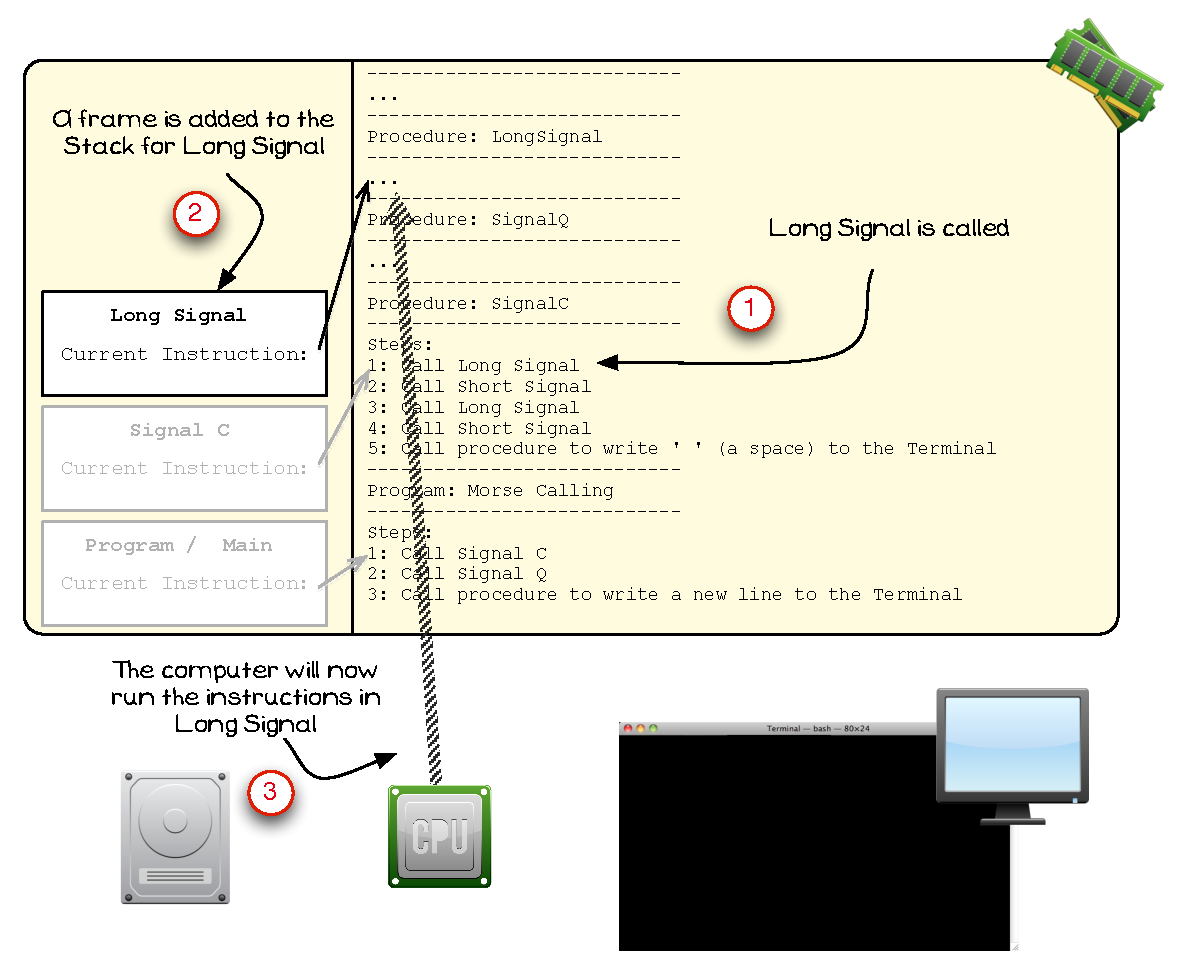
\includegraphics[width=\textwidth]{./topics/procedure-decl/images/ProcExe3} 
   \caption{Within \texttt{Signal C} the first instruction is to call \texttt{Long Signal}}
   \label{fig:procedure-decl-visualise-morsecalling-3}
\end{figure}

\mynote{
\begin{itemize}
  \item In Figure \ref{fig:procedure-decl-visualise-morsecalling-3} the indicated areas show the following:
  \begin{enumerate}
    \item The first instruction in the \texttt{Signal C} is a call to \texttt{Long Signal}.
    \item When this is executed a frame is added to the Stack to keep track of the current instruction within \texttt{Long Signal}'s code.
    \item As \texttt{Long Signal} is now on top of the Stack its instructions are executed.
  \end{enumerate}
  \bigskip
  
  \item Notice that the previous Stack Frames remain on the Stack to keep track of where the instructions return when \texttt{Long Signal} and \texttt{Signal C} finish.
  \item The computer runs each instruction one at a time, using the stack to remember where to return when the current Procedure ends.
  \item If you look at the Stack you can see that \texttt{Main} called \texttt{Signal C} that called \texttt{Long Signal}. Flip back and have a look at the \nameref{fig:procedure-decl-morsecalling-sequence}, notice that the arrows at the start of the diagram match the current state of the Stack.
\end{itemize}
}

% subsubsection long_signal_is_called (end)

\clearpage
\subsubsection{Control Returns to Signal C} % (fold)
\label{ssub:control_returns_to_signal_c}

When \texttt{Long Signal} finishes running, it has written an underscore to the Terminal, and control returns back to \texttt{Signal C}.

\begin{figure}[htbp]
   \centering
   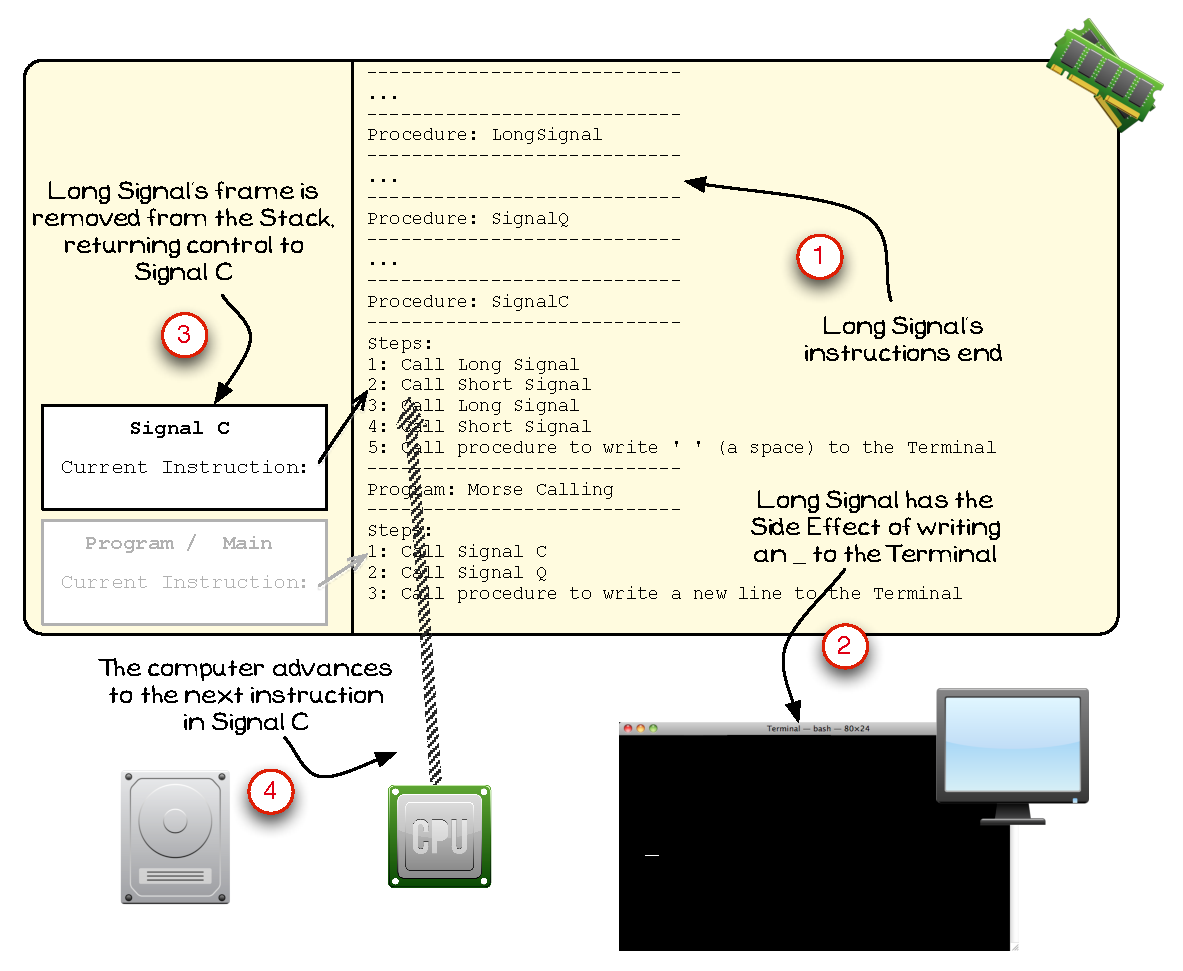
\includegraphics[width=\textwidth]{./topics/procedure-decl/images/ProcExe4} 
   \caption{\texttt{Long Signal}'s instructions end, returning control to \texttt{Signal C}}
   \label{fig:procedure-decl-visualise-morsecalling-4}
\end{figure}

\mynote{
\begin{itemize}
  \item In Figure \ref{fig:procedure-decl-visualise-morsecalling-4} the indicated areas show the following:
  \begin{enumerate}
    \item The computer runs the instructions in \texttt{Long Signal} until they end.
    \item \texttt{Long Signal} has the \textbf{side effect} of writing an underscore to the Terminal.
    \item When \texttt{Long Signal}'s instructions end control returns to \texttt{Signal C}.
    \item The computer now advanced to the next instruction in \texttt{Signal C}.
  \end{enumerate}
  \bigskip
  
  \item Procedures should have side effects, changing something as a result of being called.
  \item \texttt{Signal C} is now at its second instruction as the computer has finished its first instruction.
  \item In the \nameref{fig:procedure-decl-morsecalling-sequence} the program is now at the point after the first returning\footnote{The dashed arrow returned back from \texttt{Long Signal}.} arrow and is now about to call \texttt{Short Signal}.
\end{itemize}
}


% subsubsection control_returns_to_signal_c (end)

\clearpage
\subsubsection{Short Signal is Called} % (fold)
\label{ssub:short_signal_is_called}

The second action in \texttt{Signal C} is to call \texttt{Short Signal}.

\begin{figure}[htbp]
   \centering
   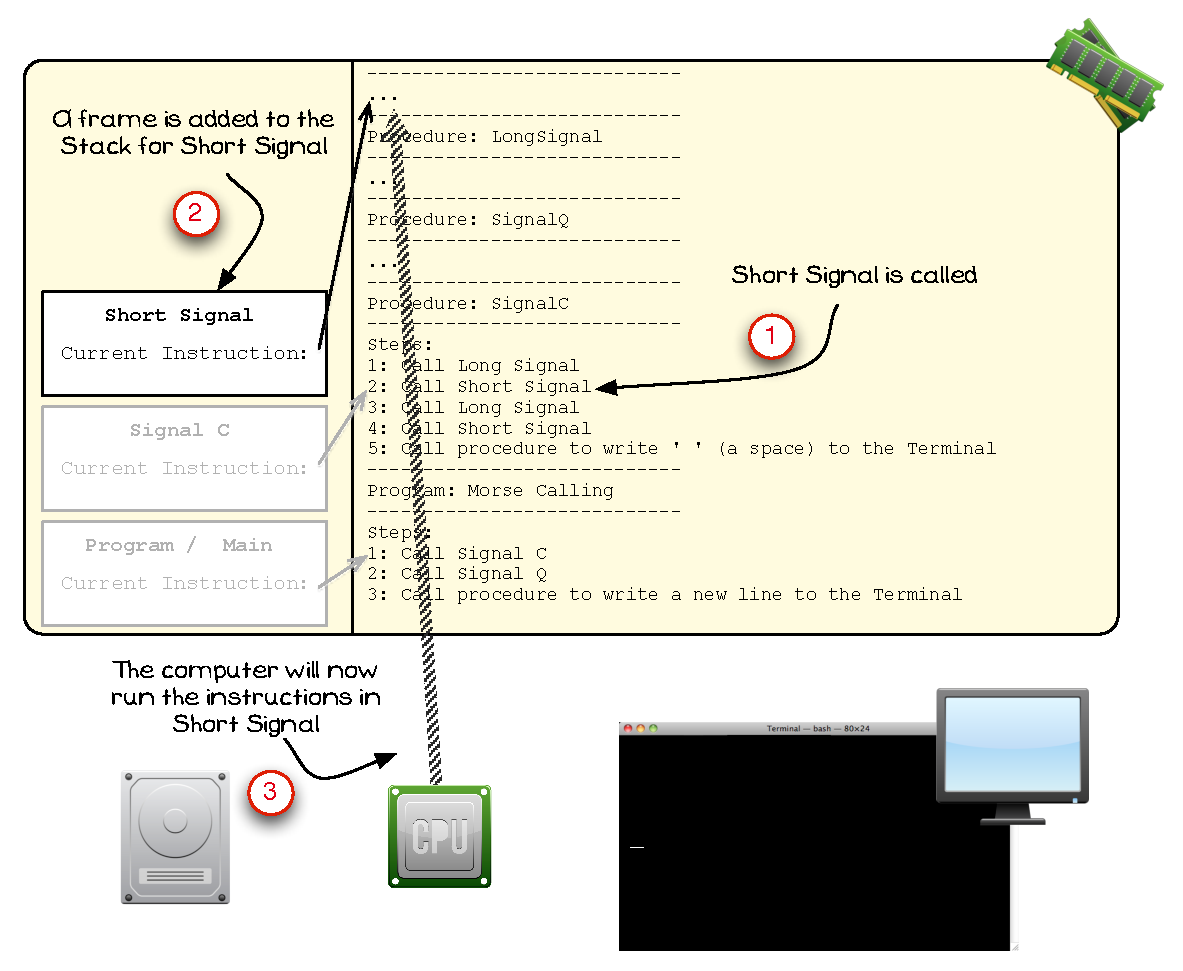
\includegraphics[width=\textwidth]{./topics/procedure-decl/images/ProcExe5} 
   \caption{\texttt{Short Signal} is called}
   \label{fig:procedure-decl-visualise-morsecalling-5}
\end{figure}

\mynote{
\begin{itemize}
  \item In Figure \ref{fig:procedure-decl-visualise-morsecalling-5} the indicated areas show the following:
  \begin{enumerate}
    \item The second instruction in the \texttt{Signal C} is a call to \texttt{Short Signal}.
    \item When this is executed a frame is added to the Stack to keep track of the current instruction within \texttt{Short Signal}'s code.
    \item As \texttt{Short Signal} is now on top of the Stack its instructions are executed.
  \end{enumerate}
  \bigskip
  
  \item In the \nameref{fig:procedure-decl-morsecalling-sequence} the program is now in the call to \texttt{Short Signal}.
\end{itemize}
}

% subsubsection short_signal_is_called (end)

\clearpage
\subsubsection{Short Signal Ends} % (fold)
\label{ssub:short_signal_ends}

When \texttt{Short Signal} ends control returns again to \texttt{Signal C}, with \texttt{Short Signal} having output a . to the Terminal.

\begin{figure}[htbp]
   \centering
   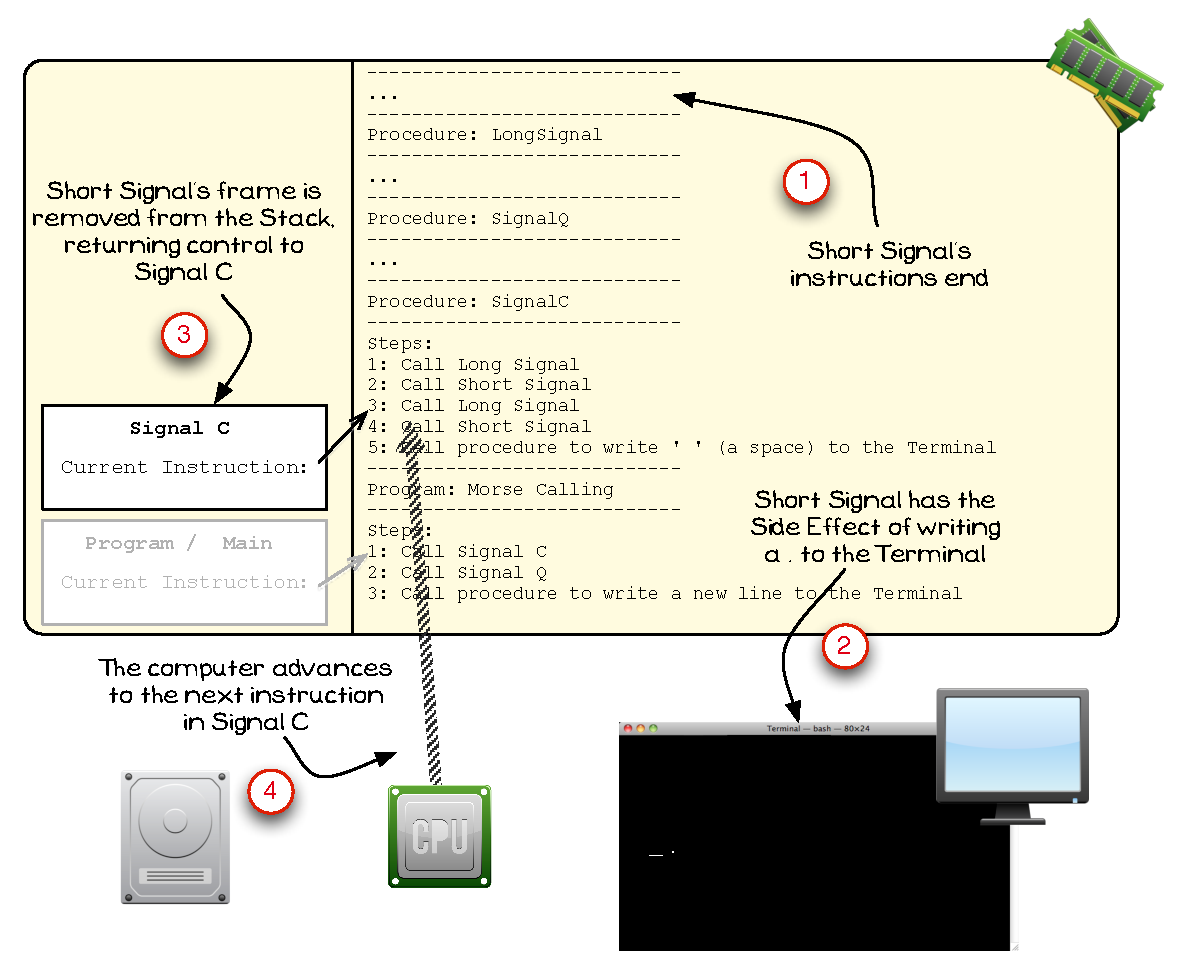
\includegraphics[width=\textwidth]{./topics/procedure-decl/images/ProcExe6} 
   \caption{\texttt{Short Signal} ends, returning control to \texttt{Signal C} again}
   \label{fig:procedure-decl-visualise-morsecalling-6}
\end{figure}

\mynote{
\begin{itemize}
  \item In Figure \ref{fig:procedure-decl-visualise-morsecalling-6} the indicated areas show the following:
  \begin{enumerate}
    \item The computer runs the instructions in \texttt{Short Signal} until they end.
    \item \texttt{Short Signal} has the \textbf{side effect} of writing an dot to the Terminal.
    \item When \texttt{Short Signal}'s instructions end control returns to \texttt{Signal C}.
    \item The computer now advanced to the next instruction in \texttt{Signal C}, the third Statement in the code.
  \end{enumerate}
\end{itemize}
}

% subsubsection short_signal_ends (end)

\clearpage
\subsubsection{Signal C runs to completion} % (fold)
\label{ssub:signal_c_runs_to_completion}

\texttt{Signal C} continues to run until it reaches the end of its instructions.

\begin{figure}[htbp]
   \centering
   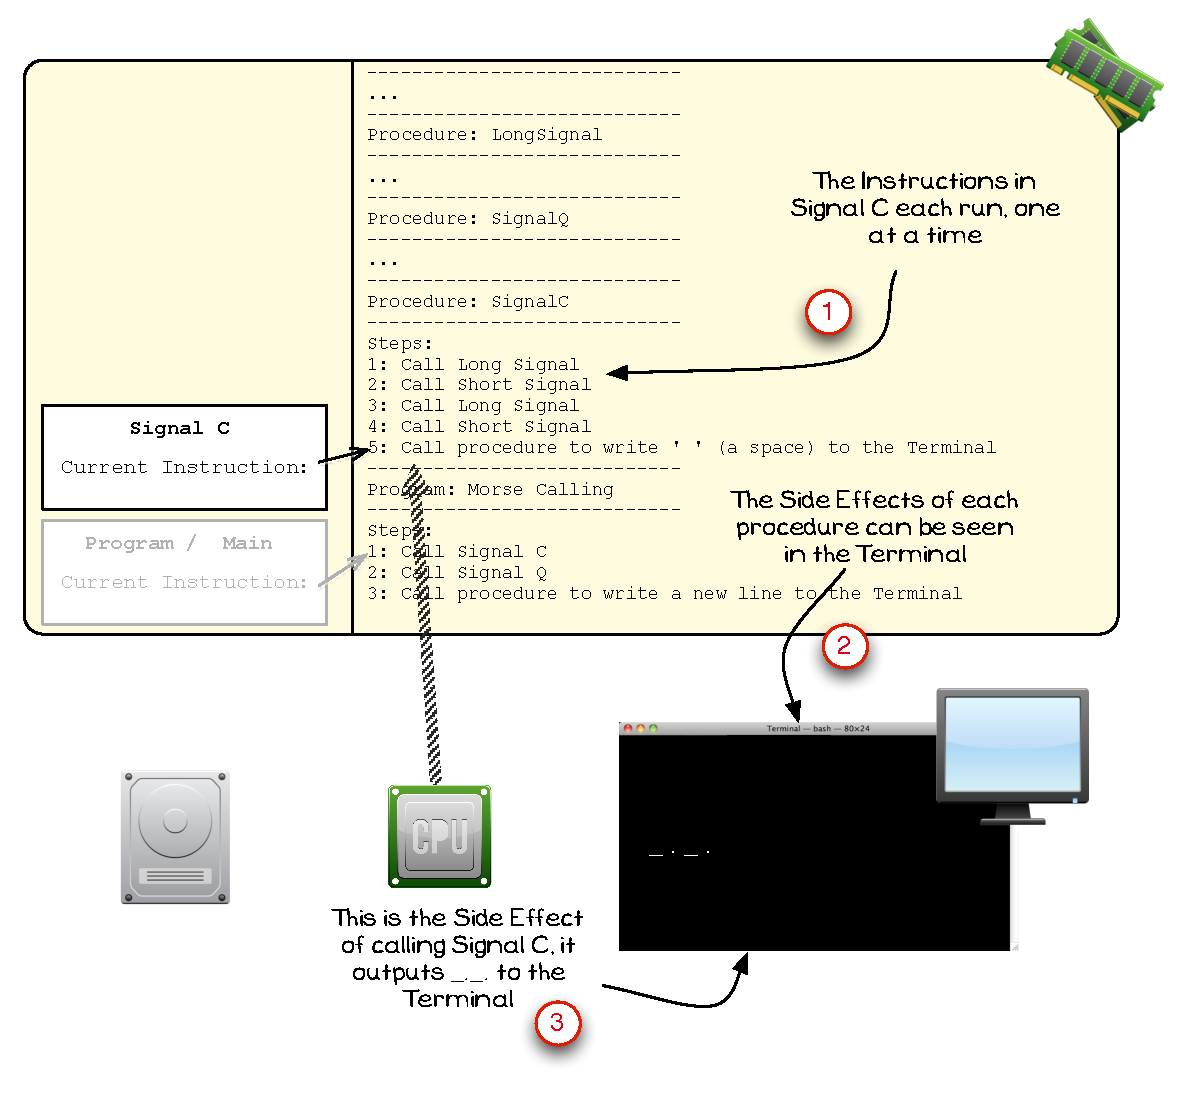
\includegraphics[width=\textwidth]{./topics/procedure-decl/images/ProcExe7} 
   \caption{\texttt{Signal C} runs until its instructions end}
   \label{fig:procedure-decl-visualise-morsecalling-7}
\end{figure}

\mynote{
\begin{itemize}
  \item In Figure \ref{fig:procedure-decl-visualise-morsecalling-7} the indicated areas show the following:
  \begin{enumerate}
    \item Each instruction in \texttt{Signal C} is run until all of the instructions in \texttt{Signal C} are complete.
    \item The side effects of the calls to \texttt{Long Signal} and \texttt{Short Signal} can be seen in the Terminal.
    \item The final state of the Terminal, showing {\morse C}, shows the side effect of calling \texttt{Signal C}.
  \end{enumerate}
\end{itemize}
}

% subsubsection signal_c_runs_to_completion (end)

\clearpage
\subsubsection{Signal Q is Called} % (fold)
\label{ssub:signal_q_is_called}

When \texttt{Signal C} finished the computer returns to the Program's main instructions, where it moves on to the call to \texttt{Signal Q}.

\begin{figure}[htbp]
   \centering
   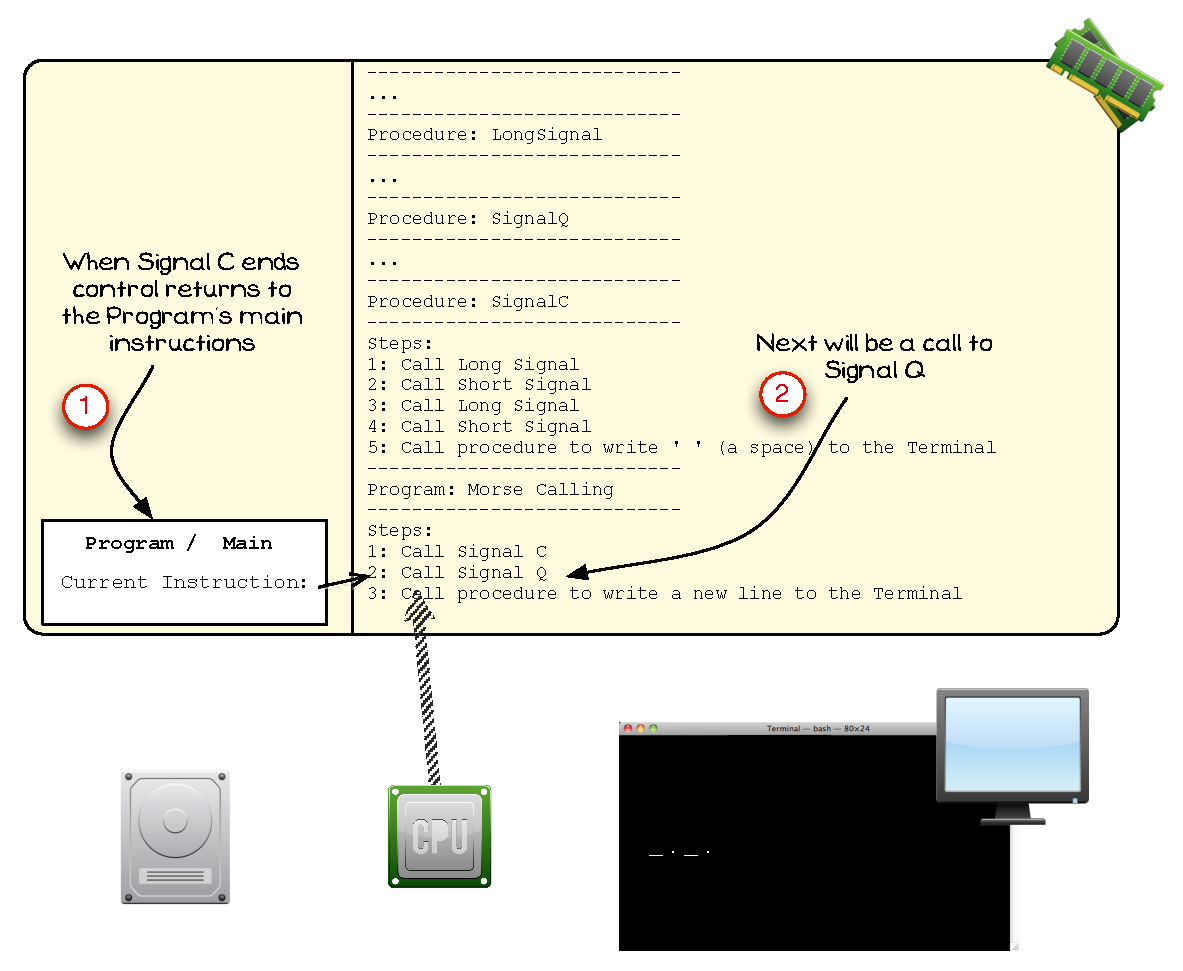
\includegraphics[width=\textwidth]{./topics/procedure-decl/images/ProcExe8} 
   \caption{}
   \label{fig:procedure-decl-visualise-morsecalling-8}
\end{figure}

\mynote{
\begin{itemize}
  \item In Figure \ref{fig:procedure-decl-visualise-morsecalling-8} the indicated areas show the following:
  \begin{enumerate}
    \item When \texttt{Signal C} ends its frame is removed from the Stack and control returns to the Program's main instructions.
    \item The next call will be to \texttt{Signal Q}. The code in \texttt{Signal Q} will run, and output {\morse Q} to the Terminal, with each of the individual characters being written by the calls to \texttt{Long Signal} and \texttt{Short Signal} in the same way as it occurred in \texttt{Signal C}.
  \end{enumerate}
  
  \bigskip
  \item If you look at the \nameref{fig:procedure-decl-morsecalling-sequence} you can see that this is the point where control has returned to main, before it calls into \texttt{Signal Q}.
\end{itemize}
}

% subsubsection signal_q_is_called (end)
% subsection visualising_procedure_calls (end)

\clearpage
\subsection{Using this to Create Procedures} % (fold)
\label{sub:using_this_to_create_procedures}

Section \ref{sub:procedure_calls_in_action}, \nameref{sub:procedure_calls_in_action}, showed the actions the computer performs in order to execute the procedures that we create, but how does this information help us create our own programs and procedures?

One important aspect about procedures is the fact that they are \textbf{isolated} from each other. Notice that \texttt{Long Signal} does not care who called it, it is responsible for performing a \emph{long signal} and carries out this task when it is called. Similarly, \texttt{Short Signal} does not care who called it, it is responsible for performing a \emph{short signal} and carries out this task when it is called. Look back at the illustrations of execution and you should be able to see each Procedure carrying out its actions before control returns to where the procedure was called. In each case the called Procedure finishes the task it is responsible for performing before it ends.

This isolation also works in the other direction. \texttt{Signal C} calls \texttt{Long Signal} when it needs a \emph{long signal} to be performed. It does not care about how \texttt{Long Signal} achieves this, and can reply upon the fact that \texttt{Long Signal} will take care of its responsibilities before it ends. When you are working on designing or coding \texttt{Signal C} you focus on the task that \texttt{Signal C} needs to perform and make use of the other Procedures without needing to worry about how these Procedures achieve their responsibilities internally.

For Software Design and Development the isolated nature of procedures means that you can, and should, focus on the Procedure you are working on and ignore details of how other procedures work internally. 


\mynote{
\begin{itemize}
  \item A Procedure has \textbf{responsibilities}. It is responsible for performing some actions to create a certain side effect.
  \item Each Procedure is \textbf{isolated} from the other code in your Program. 
  \item Focus on the Procedure you are designing or implementing, get it to meet its responsibilities and you will be one Procedure closer to your solution. Repeat this process for each Procedure in your design.
\end{itemize}
}

% subsection using_this_to_create_procedures (end)

\subsection{Summary} % (fold)
\label{sub:visualise-morse-calling-summary}

This Section has covered the use of \textbf{Structure Charts} and \textbf{Sequence Diagrams} to help visualise the relationships between procedures in a Program, and to see how these Procedures work dynamically. This was supported by the illustration of how Procedures are executed by the computer.

\mynote{
The key messages to take away from this Section are:
\begin{itemize}
  \item A Procedure has the responsibility to perform a given task.
  \item The Procedure's name should reflect the task it performs.
  \item A \textbf{Structure Chart} shows the Procedures in a Program, and how they are connected by Procedure Calls.
  \item The dynamic behaviour of the Program can be shown using a \textbf{Sequence Diagram}, this sequence of Procedure Calls within the Program.
  \item When a Procedure is called its instructions are followed. These instructions get the computer to perform the task the Procedure is responsible for.
  \item Procedures should cause \textbf{side effects}, changing something as a result of being called.
  \item Making sure each Procedure performs a \textbf{single task} will make your job easier.
  \item A \emph{single task} may have sub tasks that can be coded in their own procedures. For example, \texttt{Signal C} has sub tasks for performing long and short signals that can be coded into their own Procedures.
\end{itemize}
}

% subsection summary (end)